\section{Développement du schéma électronique} \label{sec:Dev-Schematique}
Dans cette section, nous décrirons la phase principale du développement ainsi que la démarche suivie pour élaborer le schéma électronique du projet.

\subsection{Blocs développés} \label{ssec:Dev-blocs}
Pour faciliter le développement et la lecture du schéma, il est judicieux de diviser le système en plusieurs blocs. Une structure a ainsi été définie, divisant le circuit en trois blocs principaux : \hyperref[ssec:Dev-MCU]{\textbf{Microcontrôleur \ref{ssec:Dev-MCU}}} (Intelligence du système, connexion du programmeur et LED de vie.), \hyperref[ssec:Dev-Devices]{\textbf{Périphériques \ref{ssec:Dev-Devices}}} (\gls{GNSS}, \gls{imu}, \gls{FTDI}, connecteur USB, Carte SD.) et \hyperref[ssec:Dev-Power]{\textbf{Puissance \ref{ssec:Dev-Power}}} (Connecteur batterie, gestion de charge, régulateurs de tension et système ON/OFF.).

Nous pouvons sur la figure \ref{fig:blocs} observer les différentes interaction entre les blocs, elles sont par la suite décrites dans le tableau \ref{tab:descrConnexion}.

\begin{figure}[h]
	\centering
	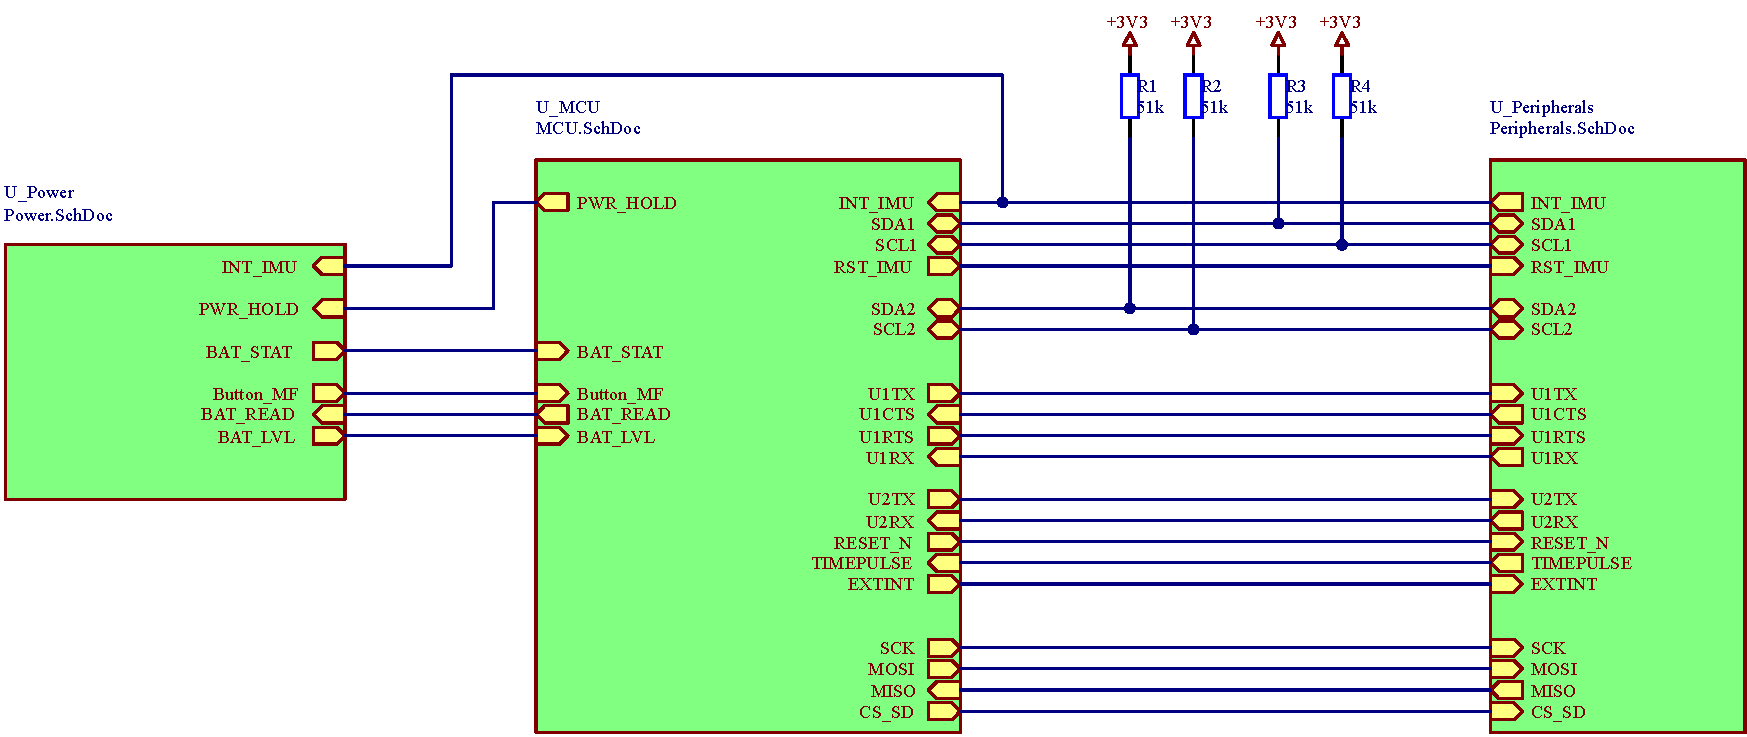
\includegraphics[width=1\linewidth]{../figures/etude/sch/BLOCS}
	\caption{Blocs du système}
	\source{Auteur}
	\label{fig:blocs}
\end{figure}

\begin{center}
	\underline{Tableau des interaction entre les blocs}
	\begin{table}[h]
		\centering
		\resizebox{\columnwidth}{!}{%
			\begin{tabular}{l|l}
				Connexion/s & Description \\
				\hline
				INT\_IMU & Interruption de la centrale inertielle, informe le \gls{mcu} et peut allumer le système. \\ 
				RST\_IMU & Permet de réinitialiser la \gls{imu}. \\
				PWR\_HOLD & Le \gls{mcu} peut se maintenir alimenté par cette connexion. \\
				BAT\_STAT & Fournit le statut de la batterie au \gls{mcu}. \\
				Button\_MF & Fournit le niveau logique du bouton au \gls{mcu}. \\
				BAT\_READ & Le \gls{mcu} peut activer la lecture de la tension de la batterie. \\
				BAT\_LVL & Lecture analogique de la tension de batterie. \\
				SDA1, SCL1 & Communication I2C avec l'\gls{imu}. \\
				SDA2, SCL2 & Communication I2C optionnelle avec le \gls{GNSS}. \\
				U1TX/RX... & Communication UART avec le \gls{FTDI} pour l'USB. \\
				U2TX/RX & Communication UART avec le \gls{GNSS}. \\
				SCK, MOSI... & Communication SPI avec la carte SD. \\ 
				R1,2,3,4 & Résistances de PULL-UP pour communication I2C. \\
			\end{tabular}
		}
		\caption{Description des connexions}
		\label{tab:descrConnexion}
	\end{table}
\end{center}

\clearpage

\subsection{Microcontrôleur} \label{ssec:Dev-MCU}

\subsubsection{Connexion} 
Pour utiliser le microcontrôleur, il est nécessaire de définir ses entrées/sorties en se référant à son \gls{datasheet}. Ce dernier permet de connaître les connexions dédiées à certains bus de communication ou à des entrées analogiques. 

\begin{figure}[h]
	\centering
	\begin{subfigure}[b]{0.7\textwidth}
		\centering
		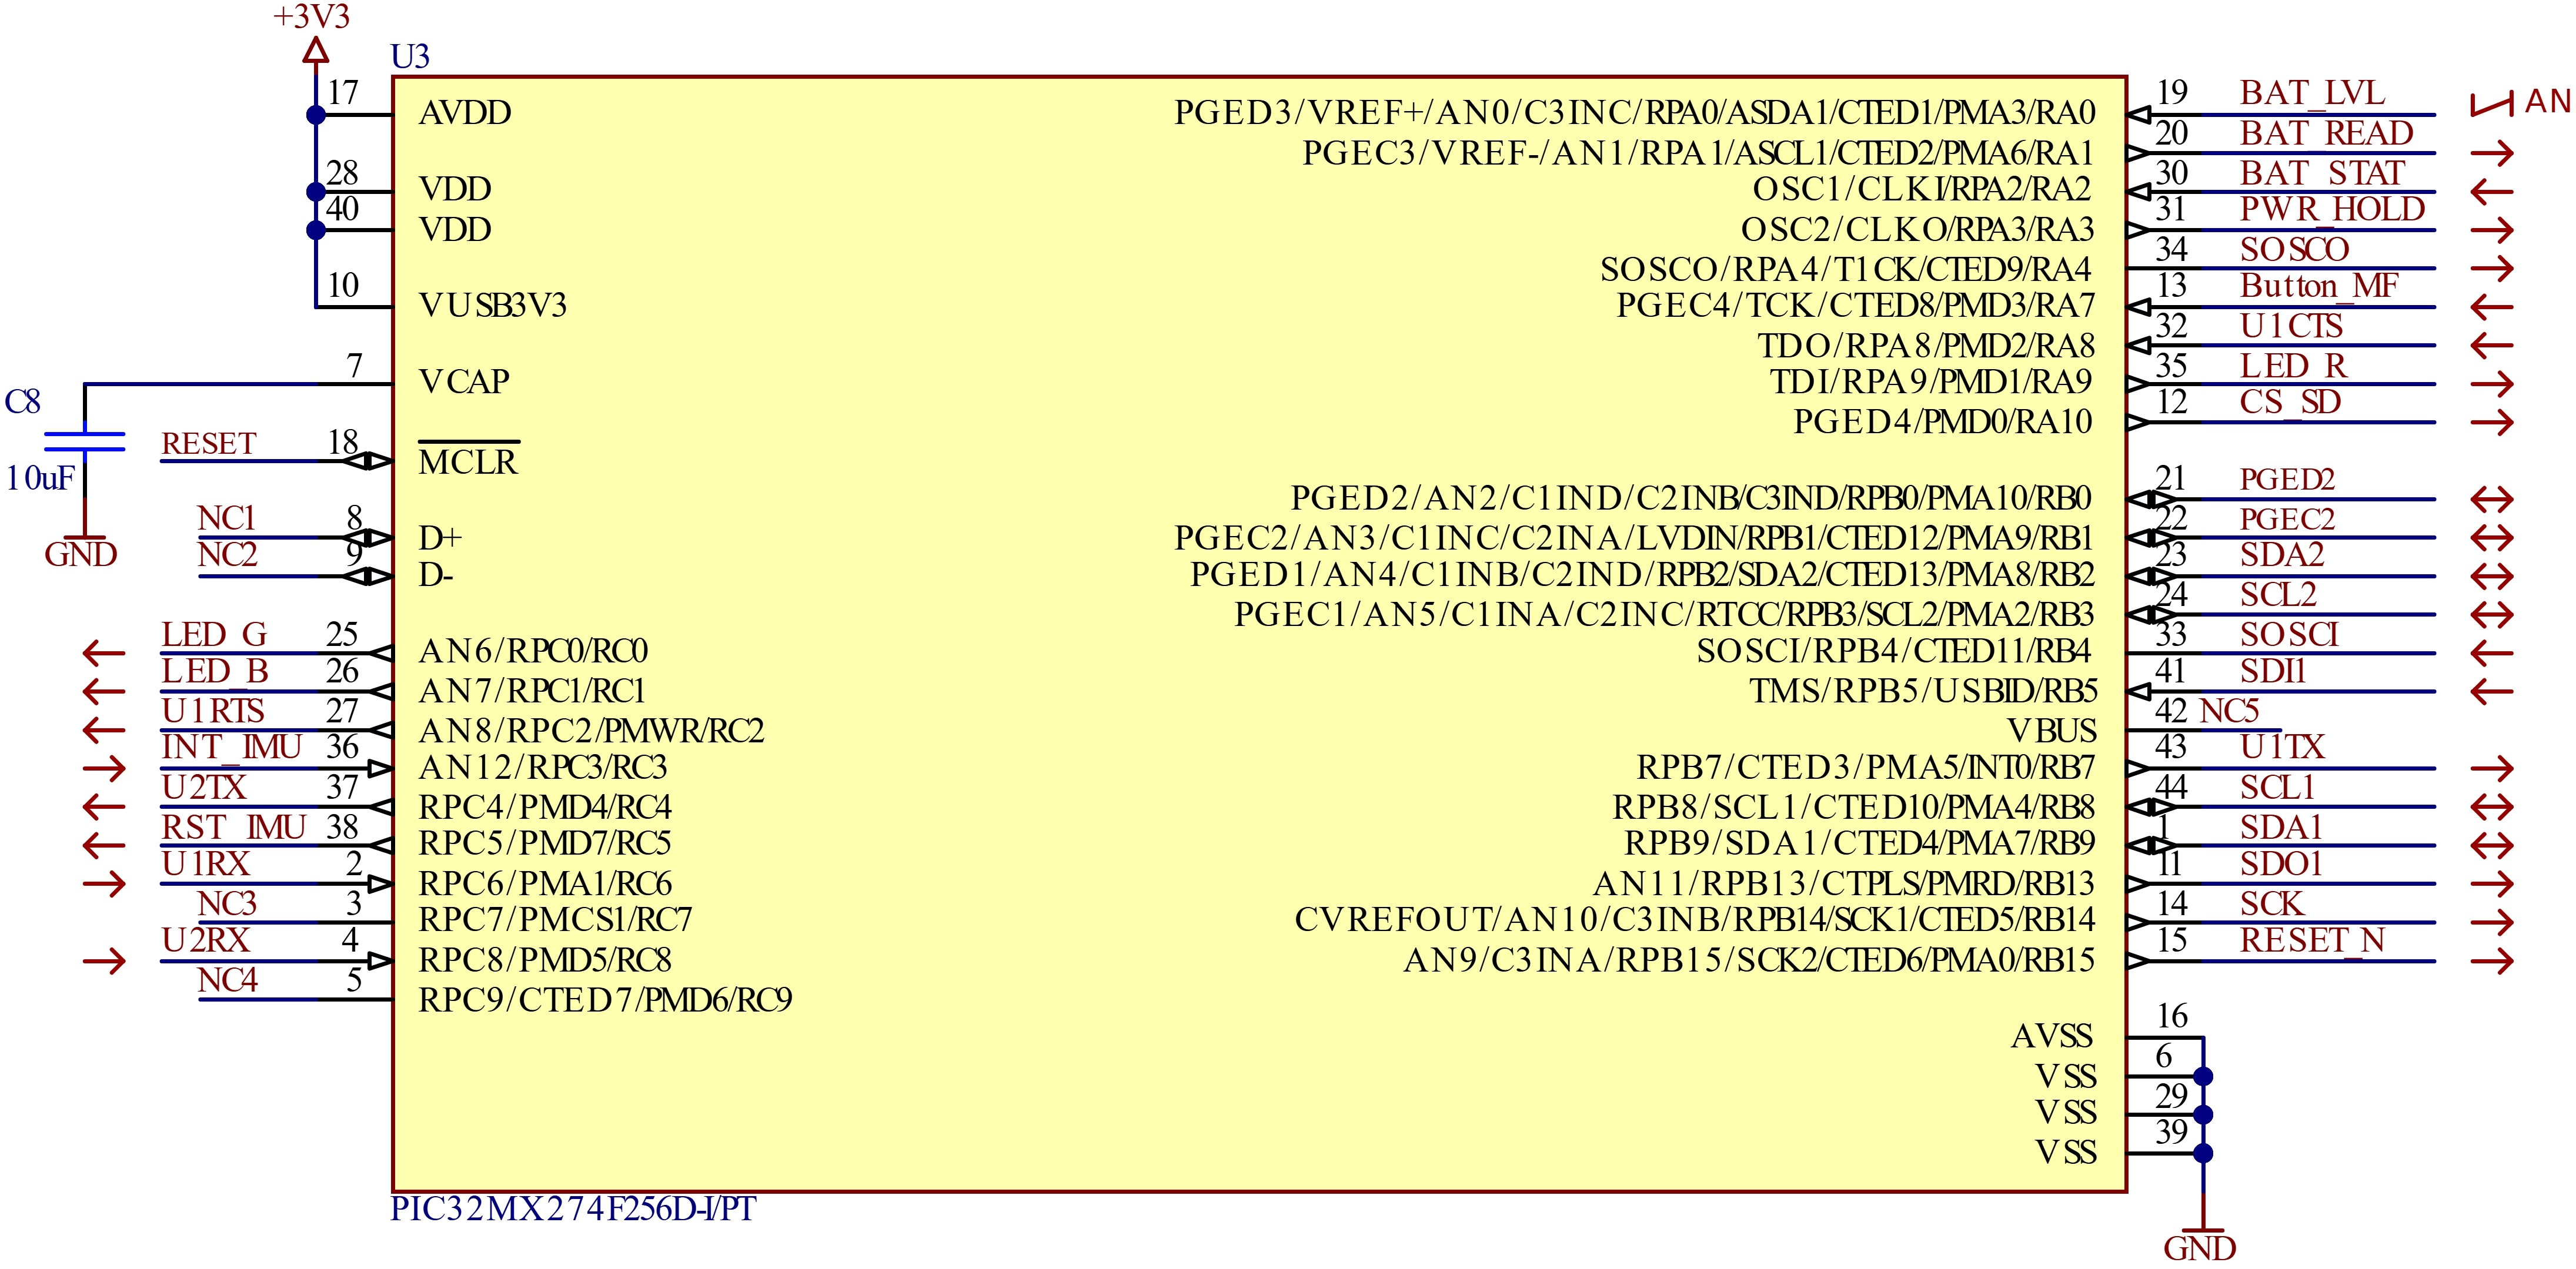
\includegraphics[width=1\linewidth]{../figures/etude/sch/MCU}
		\caption{Connexions du microcontrôleur}
		\label{fig:mcu}
	\end{subfigure}
	\hfill
	\begin{subfigure}[b]{0.25\textwidth}
		\centering
		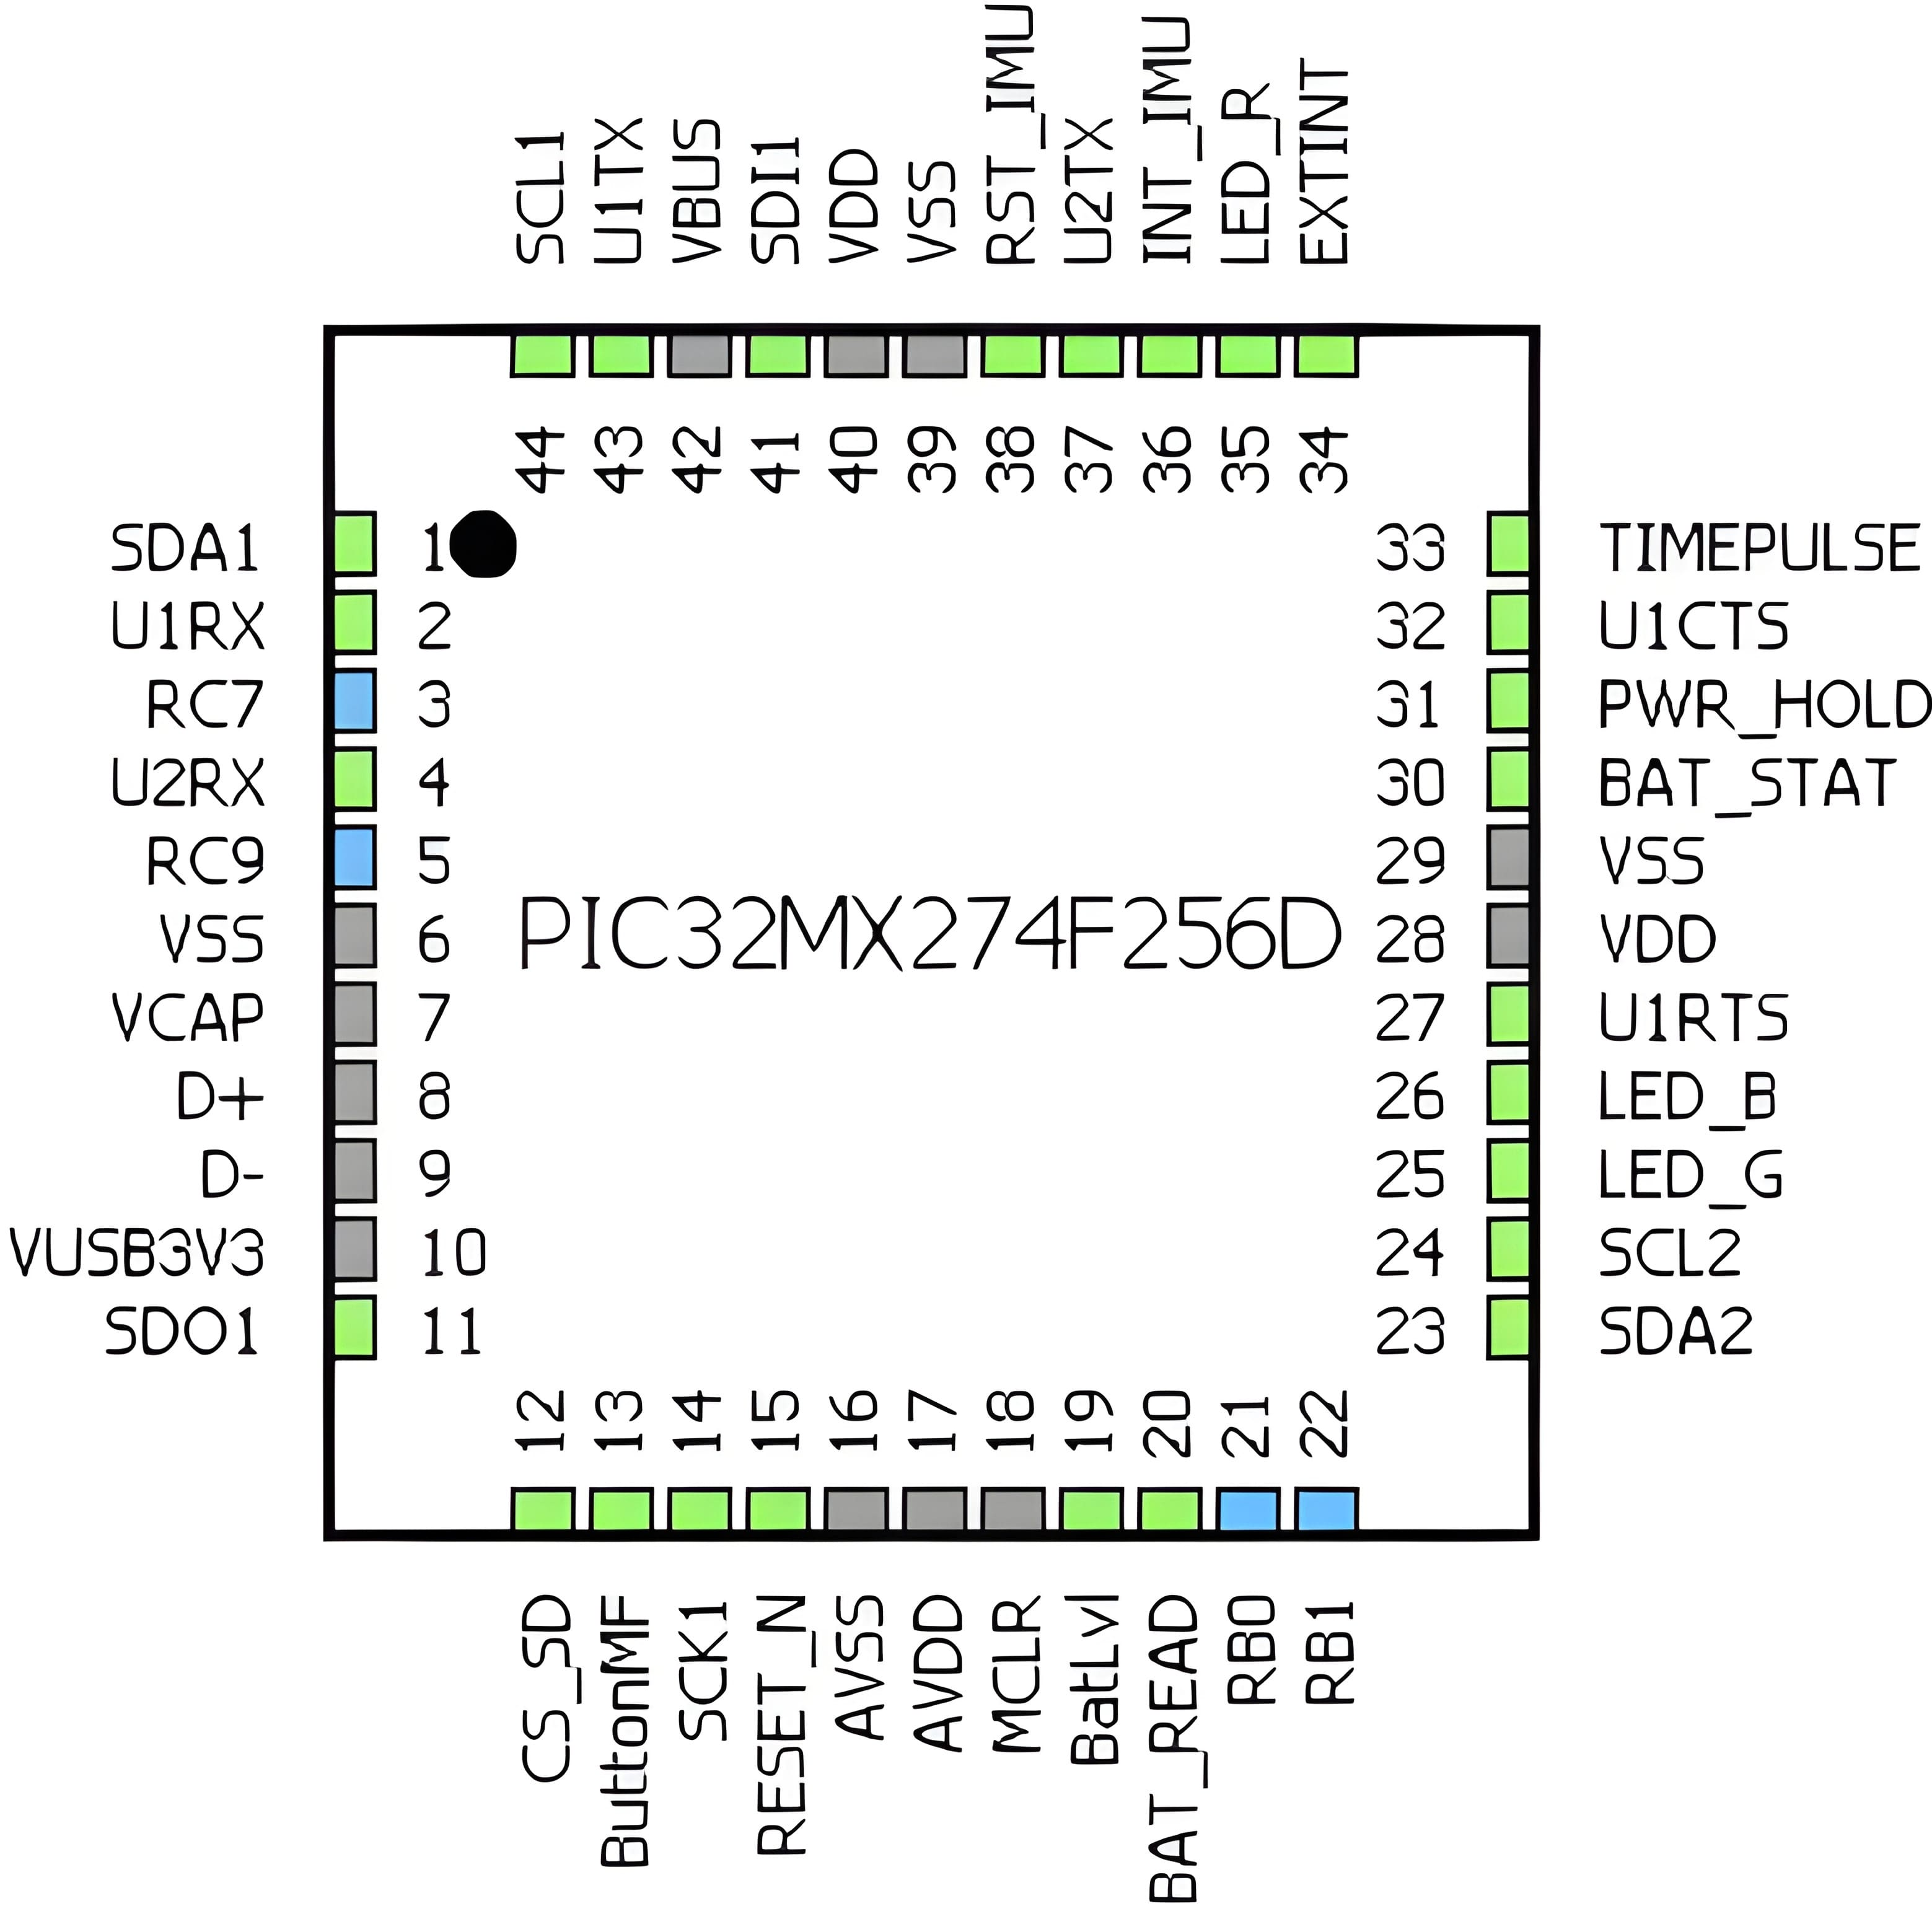
\includegraphics[width=1\linewidth]{../figures/etude/sch/MCU-HARMONY}
		\caption{Config. \gls{harmony}.}
		\label{fig:mcu-harmony}
	\end{subfigure}
	\hfill
	\caption{Configuration des PINs du microcontrôleur}
	\source{Auteur}
	\label{fig:sch-connMcu}
\end{figure}

Pour valider les connexions de la figure \ref{fig:mcu}, une vérification a été effectuée avec le configurateur graphique \gls{harmony}, illustrée par la figure \ref{fig:mcu-harmony}. Cette démarche a confirmé la possibilité de dédier certaines fonctions à des PINs.

\subsubsection{Programmateur et reset} 

\begin{figure}[h]
	\centering
	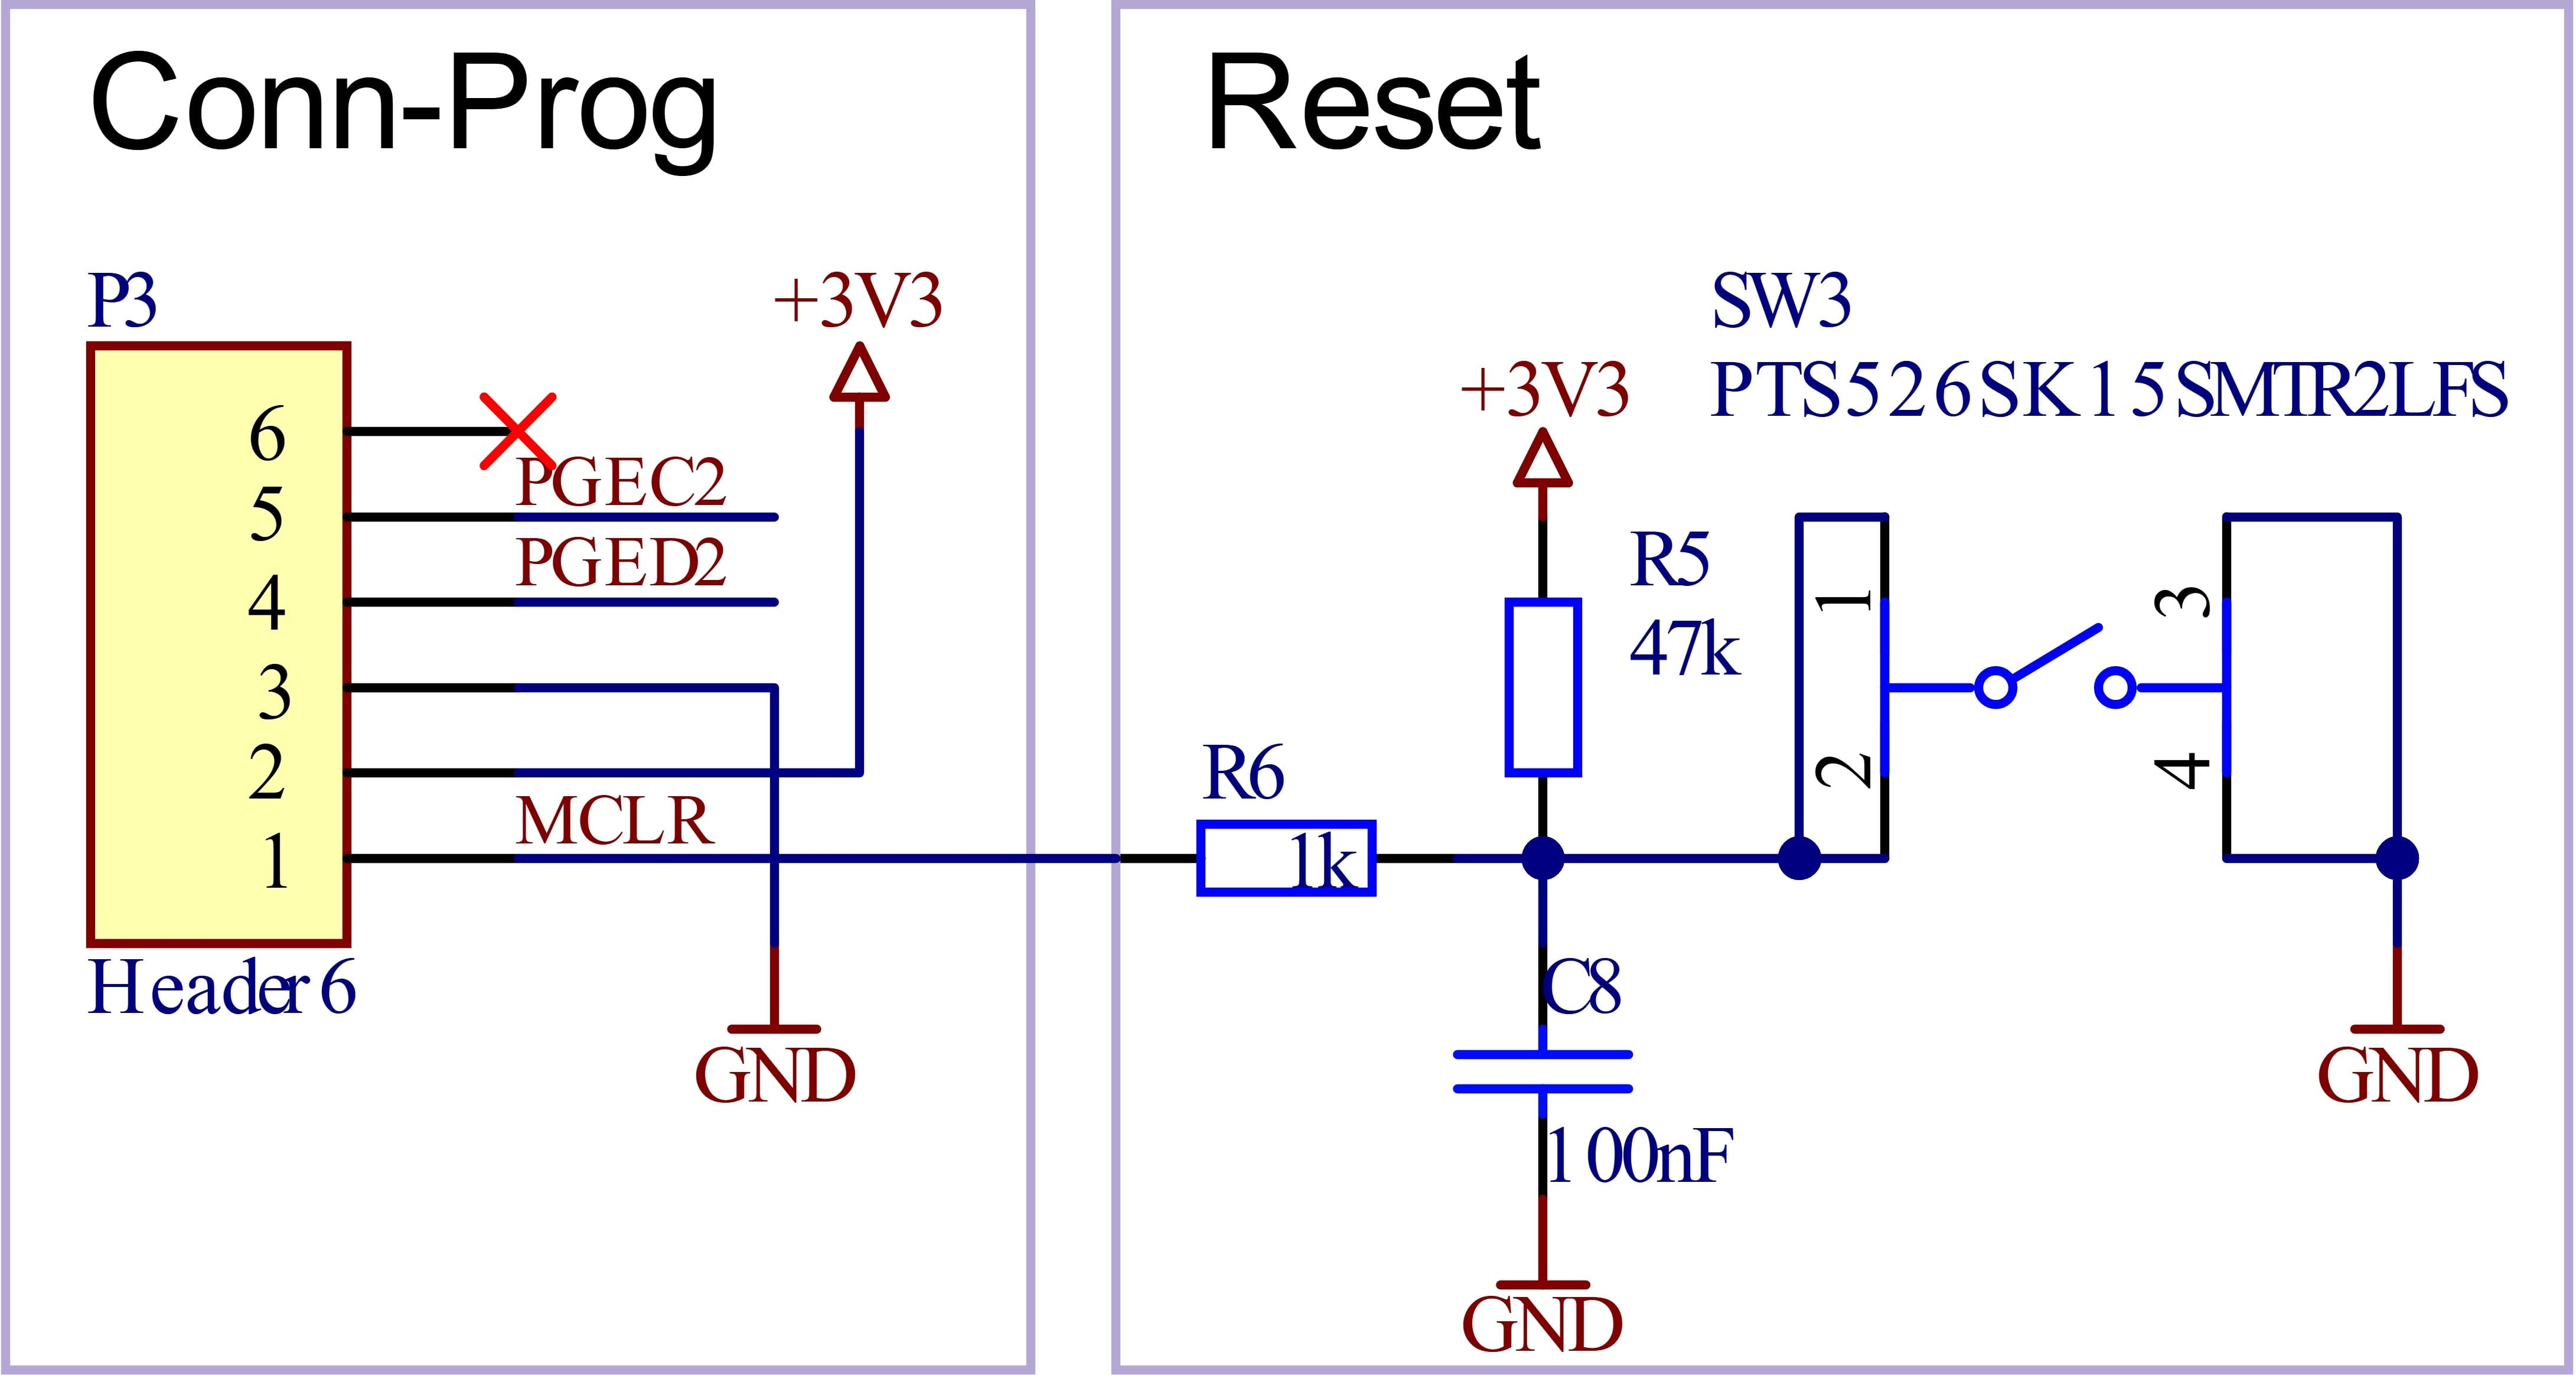
\includegraphics[width=0.7\linewidth]{../figures/etude/sch/Prog-Reset}
	\caption{Schéma programmateur et reset}
	\source{Auteur}
	\label{fig:prog-reset}
\end{figure}

Sur la figure \ref{fig:prog-reset}, nous pouvons observer le connecteur de programmation \textit{P3}. La connexion \textbf{MCLR} (Master Clear), qui permet de réinitialiser le \gls{mcu} lors de sa programmation, est suivie d'un circuit de protection du \gls{mcu} et d'un bouton pour permettre une réinitialisation manuelle.

\clearpage

\subsubsection{LED de vie} 

\begin{figure}[h]
	\centering
	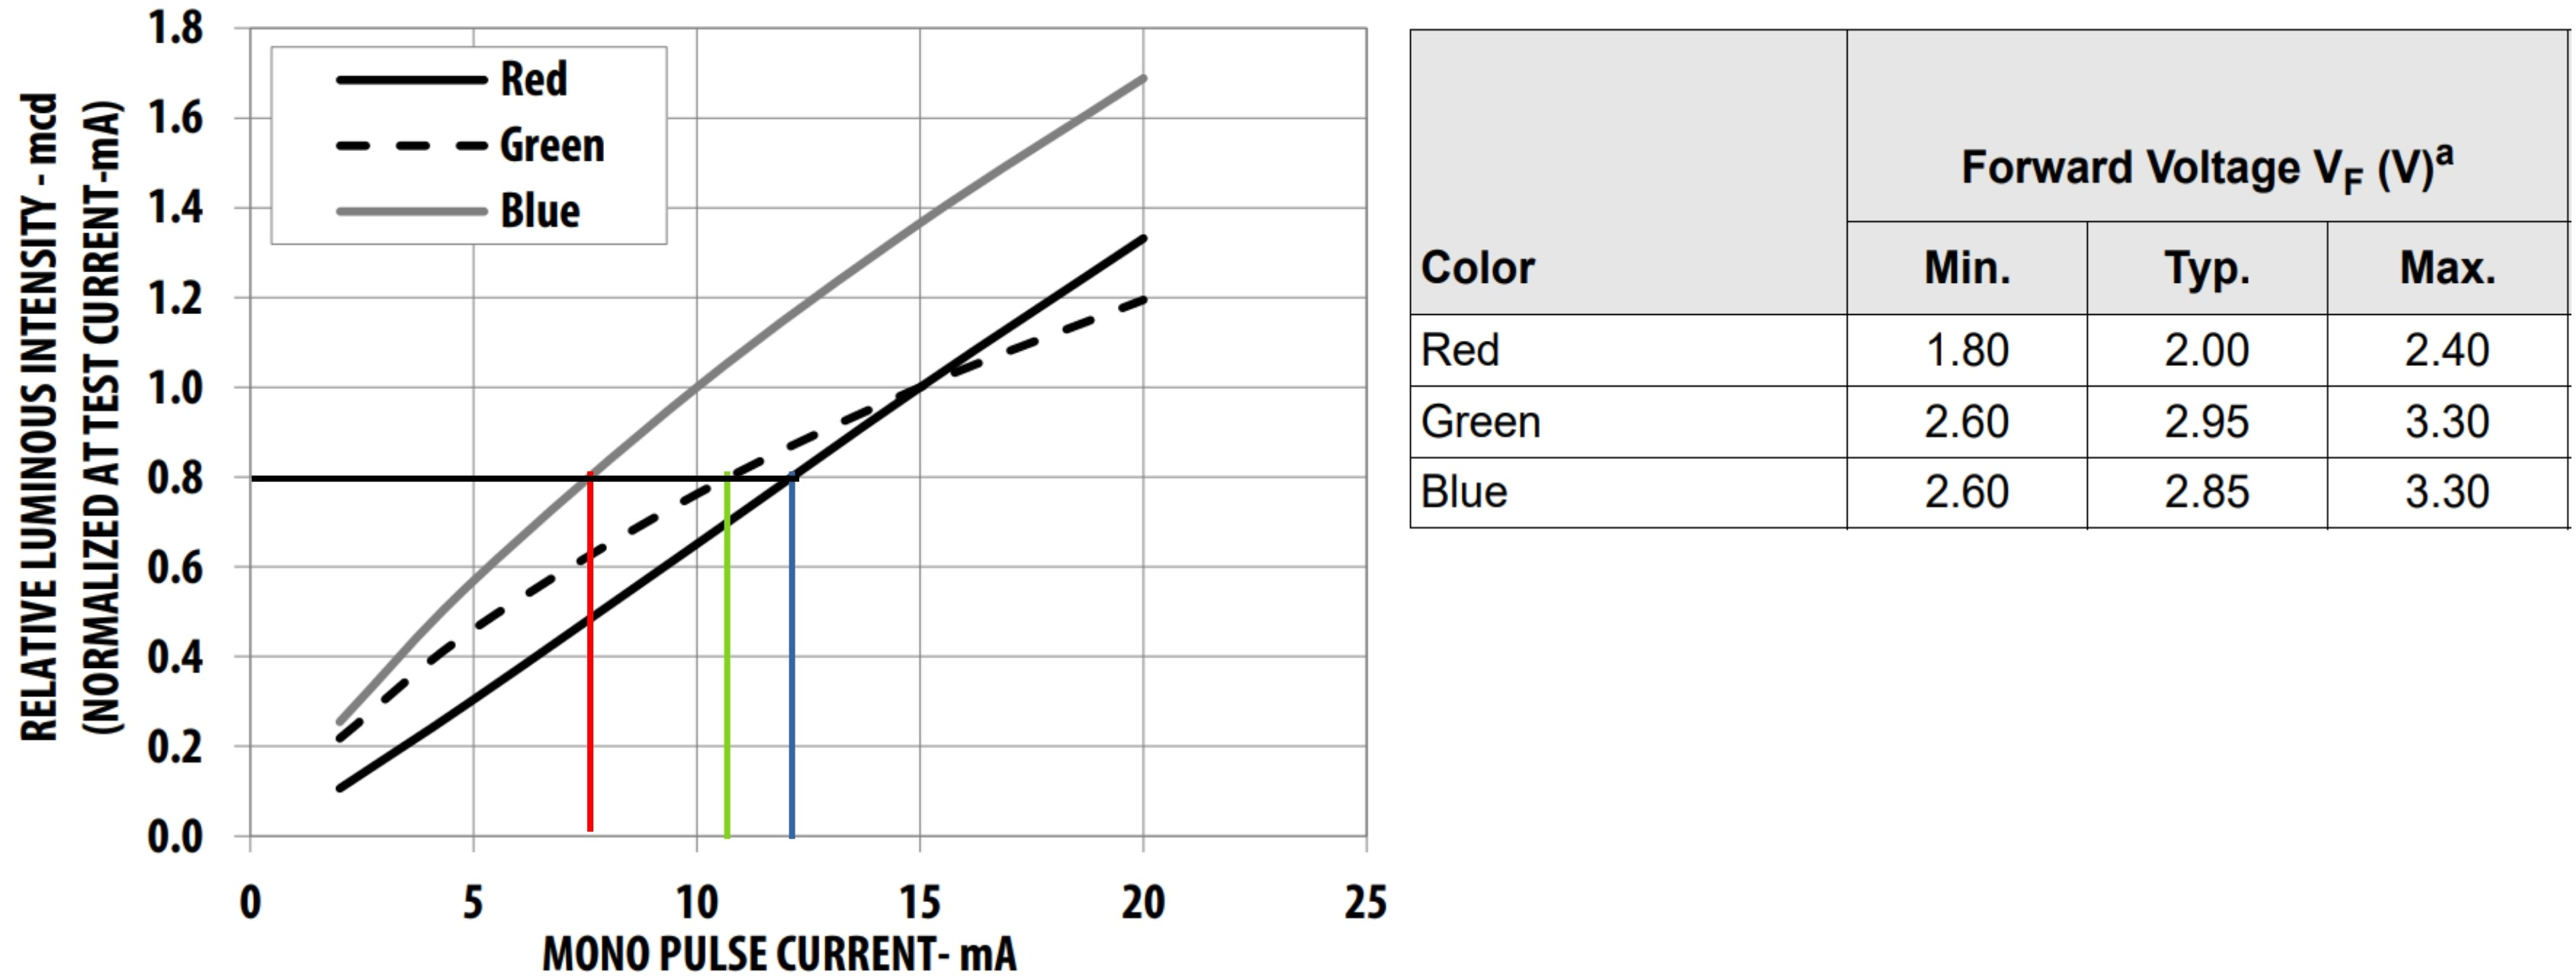
\includegraphics[width=.8\linewidth]{../figures/etude/DIM-LED}
	\caption{Données de la LED}
	\source{\gls{datasheet} \href{https://docs.broadcom.com/doc/ASMB-KTF0-0A306-DS100}{ASMB-KTF0-0A306}}
	\label{fig:dim-led}
\end{figure}

\begin{figure}[h]
	\centering
	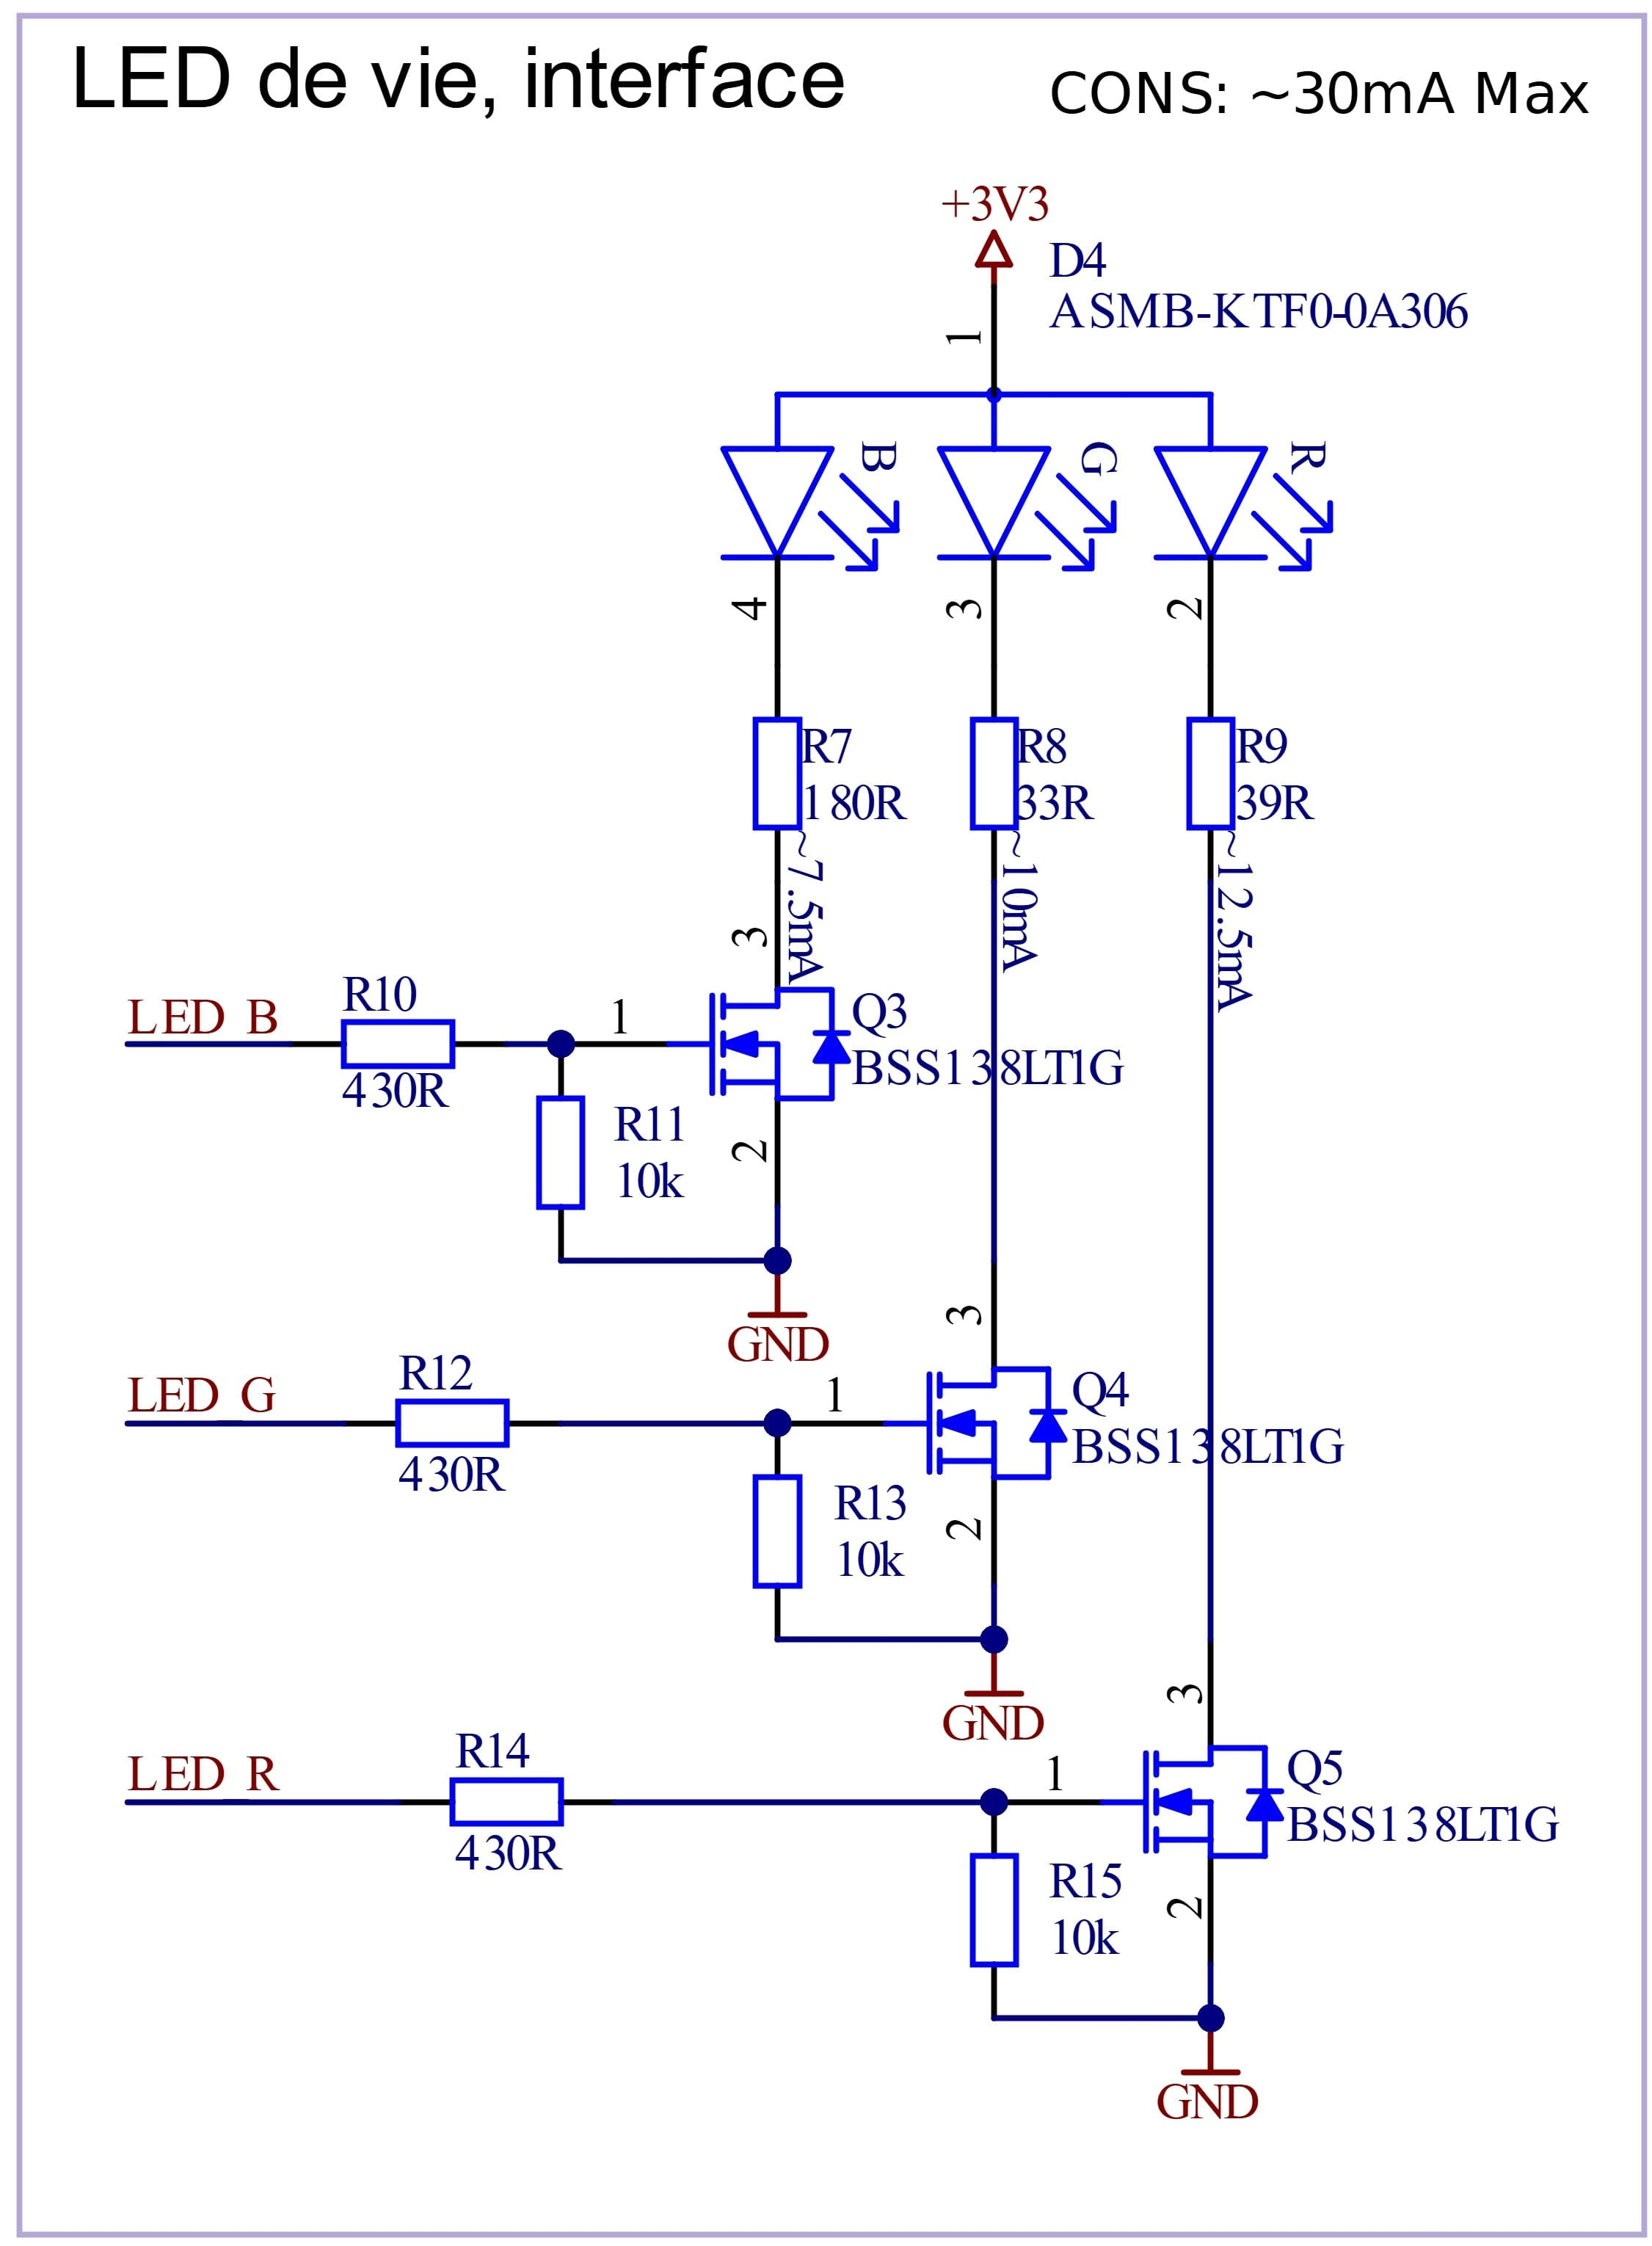
\includegraphics[width=0.4\linewidth]{../figures/etude/sch/LED-Vie}
	\caption{Schéma de la LED de vie}
	\source{Auteur}
	\label{fig:led-vie}
\end{figure}

Les résistances de la figure \ref{fig:led-vie} ont été dimensionnées en respectant les caractéristiques des LEDs pour chacune des couleurs (voir figure \ref{fig:dim-led}). Ces dernières éclairent à 80\% de leur luminosité nominale dans un souci d'économie d'énergie, leur utilité étant réduite à ce stade de prototypage.

\begin{center}
	\underline{Exemple dimensionnement résistance LED bleue}
	\begin{equation*}
		R_{blue} = \frac{(Vcc - V_{blue})}{I_b} = \frac{(3.3 - 2.85)}{12*10^-3} = 37.5 \Omega
	\end{equation*}
\end{center}

\clearpage

\subsection{Périphériques} \label{ssec:Dev-Devices}

\subsection{Puissance} \label{ssec:Dev-Power}

\subsection{Dimensionnements} \label{ssec:Dev-Dimensionnements}

\subsubsection{Bus de communications} \label{sssec:Dev-BusComm}

\subsubsection{Interface} \label{sssec:Interface}

\subsubsection{Périphériques} \label{sssec:Peripheriques}

\subsubsection{Chargeur de batterie} \label{sssec:Chargeur-bat}

\subsubsection{Adaptation mécanique} \label{sssec:Adaptation-mech}

\subsection{Synthèse et perspectives de l'étude} \label{ssec:Synth-etude}